% !TEX root = ../report.tex

\chapter{Design}

\minitoc
This chapter the architecture and components in the architecture, how they were designed, and how they fulfill the requirements of the project.


\clearpage


\section{Definitions}


\section{Architecture}
The architecture of the project is based on The 4+1 View
Model of Software Architecture \cite{Kruchten}. The views are used reflect the structural aspects, temporal aspects, technological development aspects and physical aspects of the project.

The architecture uses a custom simplified version of the 4+1 notation that better fits the descriptive needs for the project.


\subsection{Logical View}
The logical view describes the components of the architecture and how they relate to one another in terms of containment, inheritance and usage. The logical view can be found in figure-\ref{figure:logical-view} and the notation for the logical view in figure-\ref{figure:logical-view-notation}

\begin{figure}[H]
\centerline{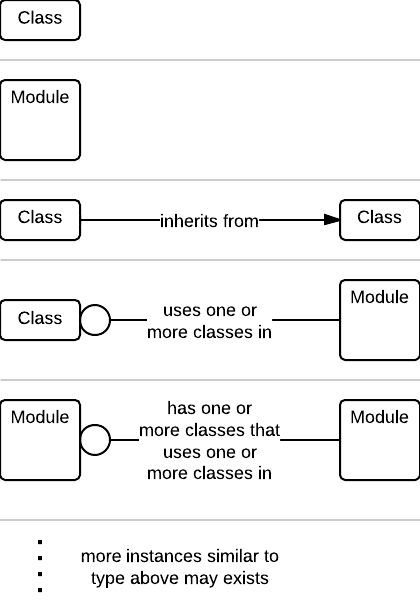
\includegraphics[width=2.5in]{image/architecture-logical-view-notation.png}}
\caption{Notation for the logical view.}
\label{figure:logical-view-notation}
\end{figure}

\begin{center}
\begin{figure}[H]
\centerline{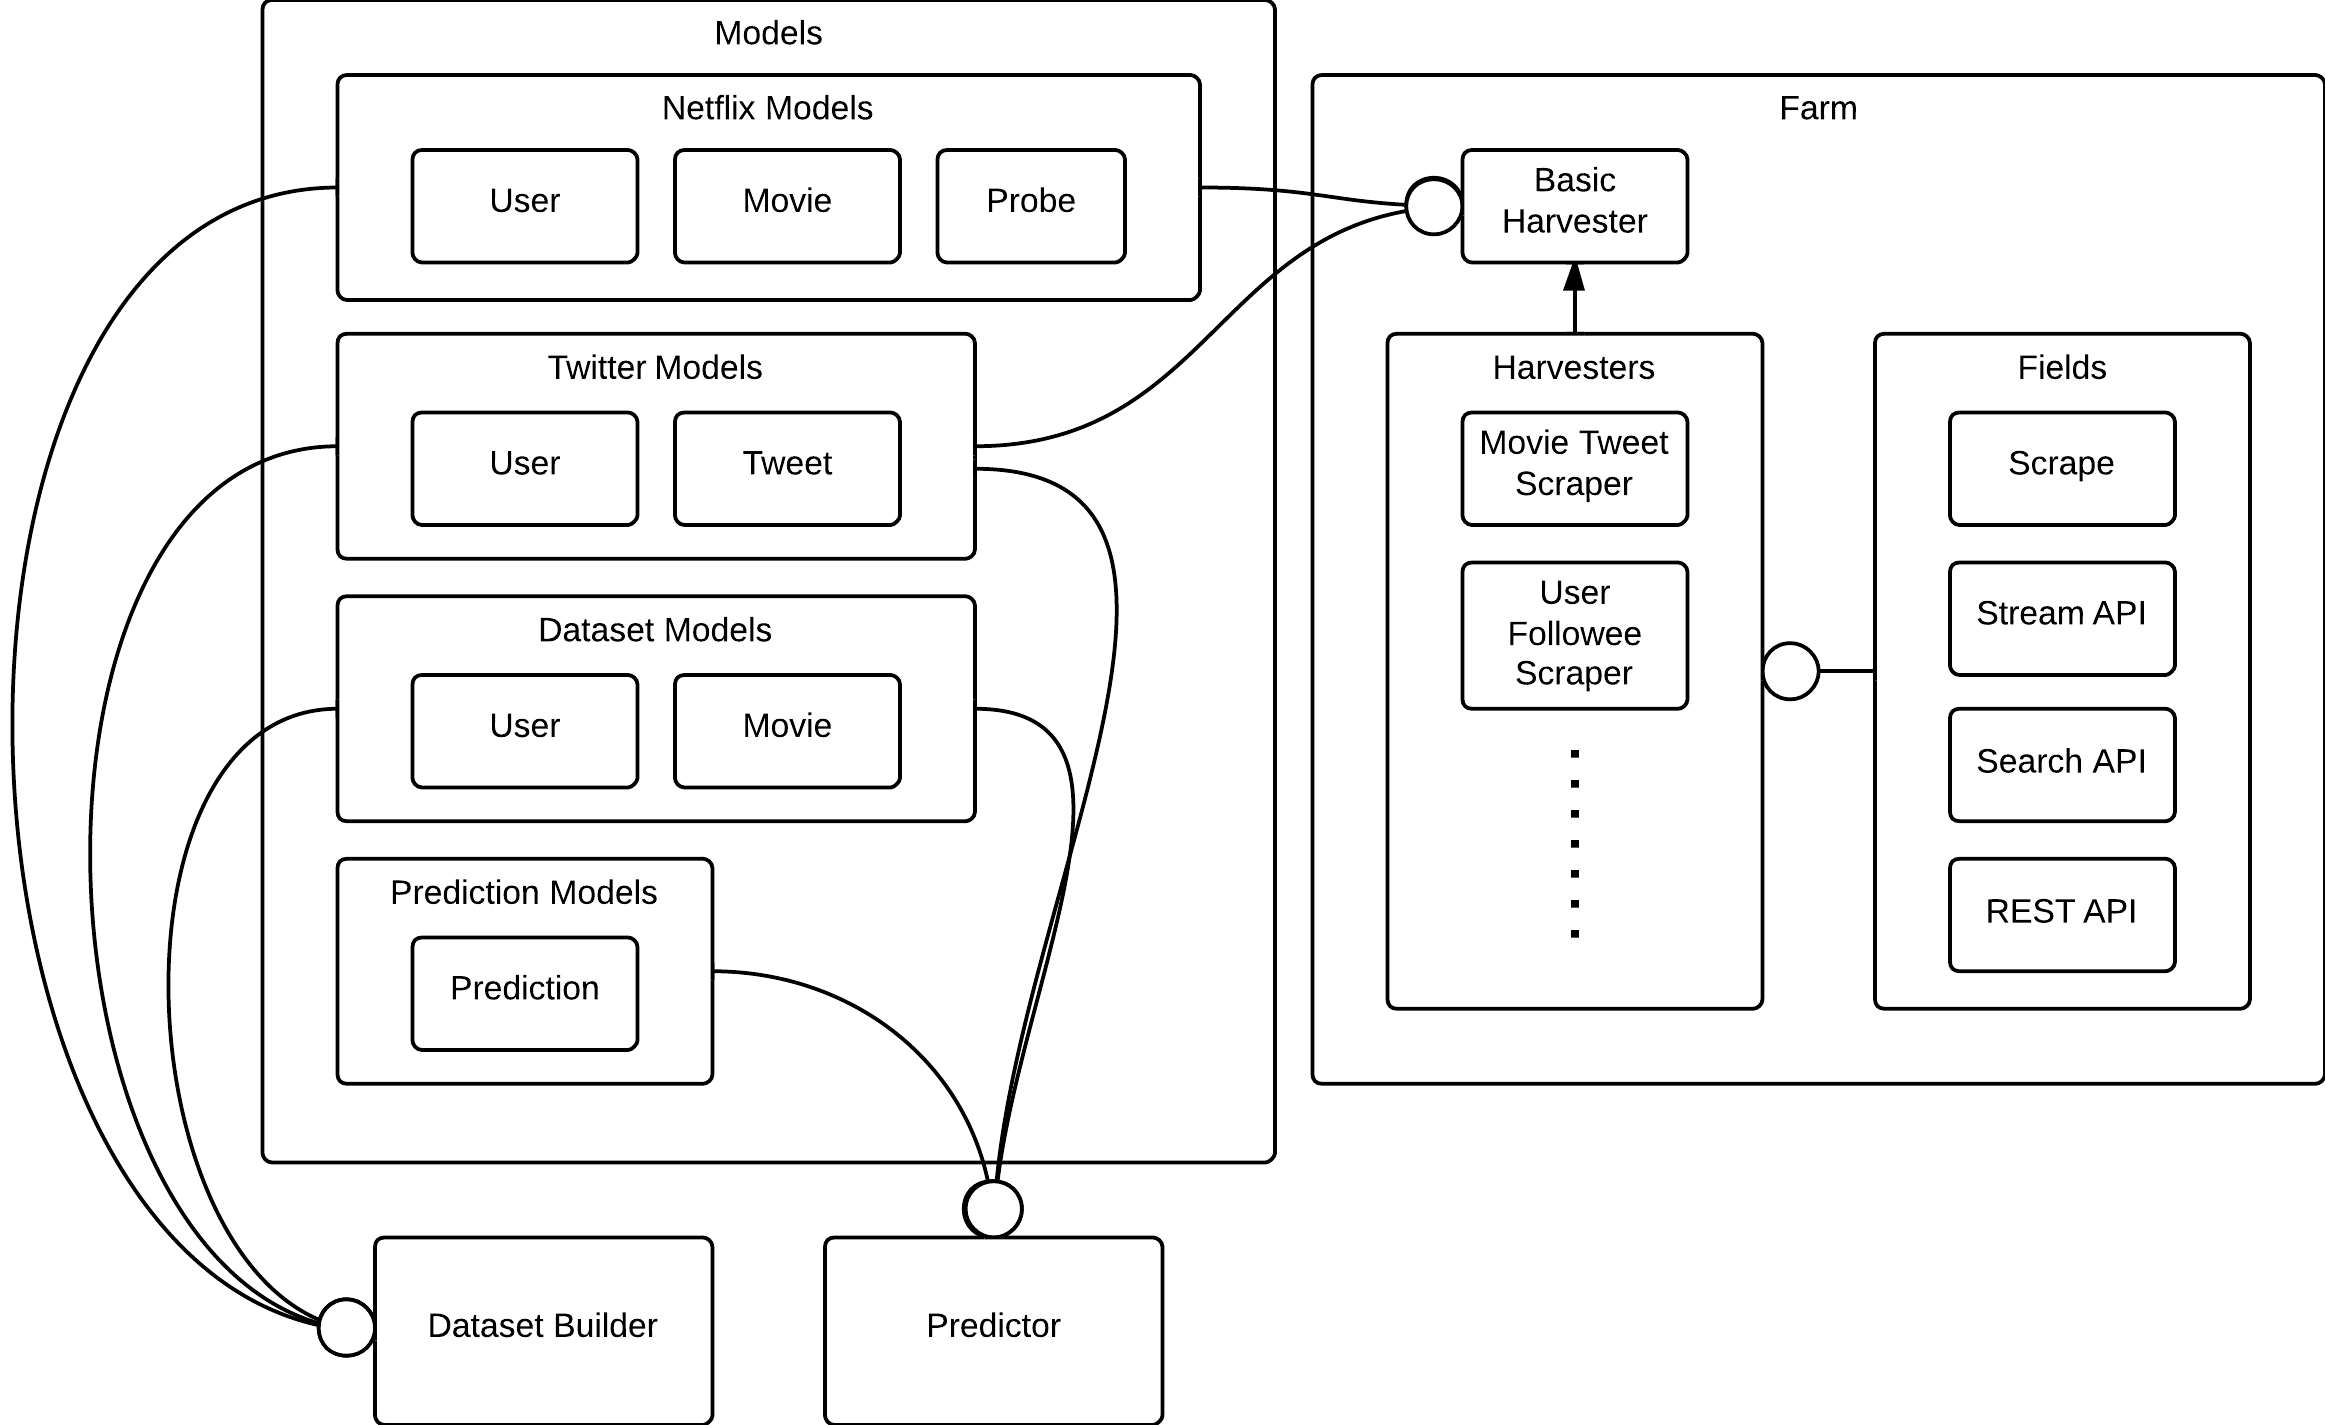
\includegraphics[width=7in]{image/architecture-logical-view.png}}
\caption{Logical view of the project. See figure-\ref{figure:logical-view-notation} for notation.}
\label{figure:logical-view}
\end{figure}
\end{center}

\subsubsection{Models}
Models is the module responsible for holding the different datamodels that are used in the project. It is found in the upper left part of the logical view in figure-\ref{figure:logical-view}. All classes in this module are mapped to and reflect the database.

The Netflix Models model the netflix prize dataset. Each user has a list of movie ratings and each movie has a list of user ratings. The probe is a list of movies with empty user ratings that need to be predicted.

The Twitter Models reflect the data harvested from Twitter. The schema of these models are variable as it depends on what type of data is harvested. A tweet typically contains a text and refers to a user. A user typically has a name and a user ID and may refer to tweets. As an example, it may also contain a list of followees or followers.

The Dataset Models reflects the Netflix Models after they have been mapped to fused with Twitter Models by the Dataset Builder.

The Prediction Models model what the ratings that the Predictor predicts using the Datast Models and the Probe in Netflix Models.

\subsubsection{Farm}


\subsubsection{Dataset Builder}

\subsubsection{Predictor}


\subsection{Process View}
The process view describes the actions that the components of the architecture engage in over time and how there actions relate to other components. See figure-\ref{figure:process-view}

\begin{figure}[H]
\centerline{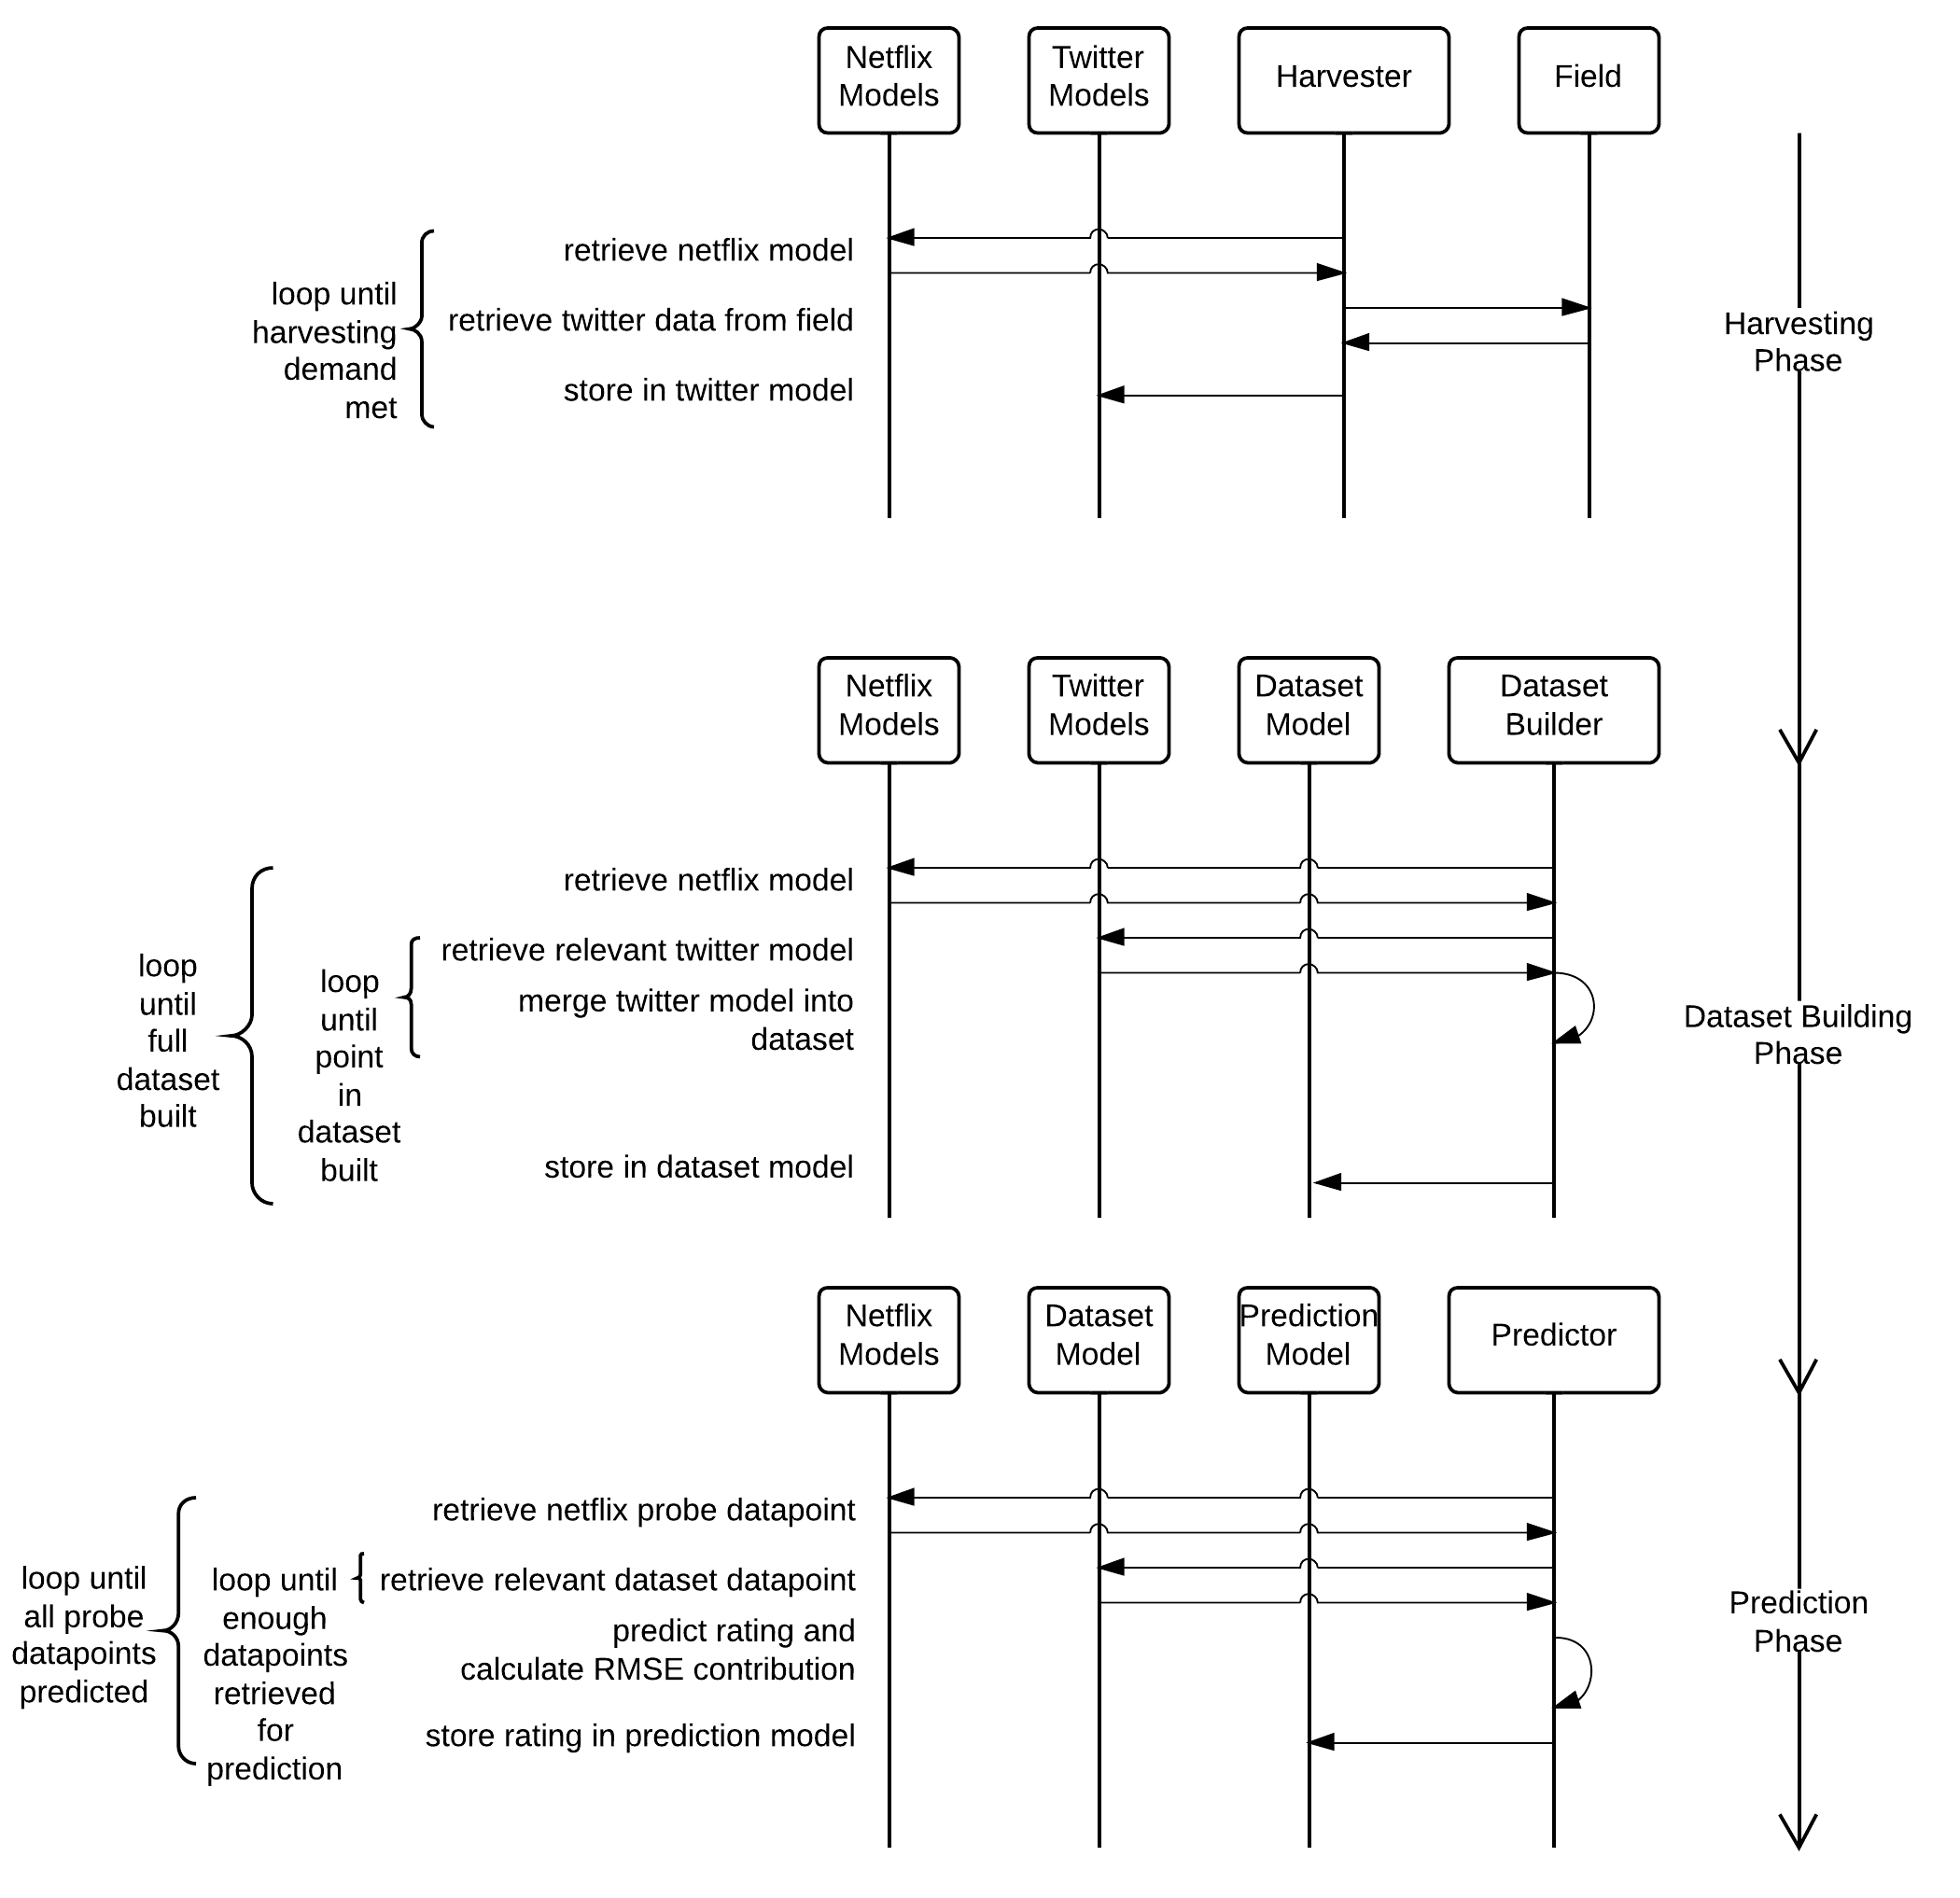
\includegraphics[width=7in]{image/architecture-process-view.png}}
\caption{Process view showing the actions taken by various components as time passes and which components they affect. Time is moving downward. An arrow implies that data is sent from one component to another. The data being sent can be a function call, an object or any other type available to the component taking the action.}
\label{figure:process-view}
\end{figure}

\subsubsection{Harvest Phase}
The harvest phase is responsible for gathering data from Twitter. First, the harvester retrieves an initial model from either netflix models or twitter models. Then, it uses one or more fields to harvest data from Twitter that is related to the initial model. This can be tweets containing the movie title in the tweet.text, tweet.users for these tweets, users.each.followees and so forth, as outlined in the functional requirements related to harvesting in section~\ref{section:functional-requirements}. At last, the harvested data is stored as twitter models.

\subsubsection{Datset Building Phase}
The dataset building phase is responsible for building a dataset using the data gathered from Twitter in the harvest phase. First, the dataset builder retrieves a netflix model, which is likely to be a movie. Then, it retrieves twitter models that are relevant for the netflix model and consolidates them into a set of datapoints that expresses this netflix model. At last, the datapoints are stored along with the netflix model it expresses in the dataset model. In this way, the functional requirement in section~\ref{section:functional-requirements} for supplementing the netflix-dataset with data from twitter is fulfilled.

\subsubsection{Prediction Phase}
The prediction phase is responsible for using the dataset model to predict the ratings of the probe in the netflix model and calculate the RMSE. First, the predictor retrieves a datapoint from the probe. Then, it gathers the relevant datapoints it needs from the dataset model in order to make a prediction. After this step, the rating has been predicted and the contribution to the RMSE score is calculated and. The RMSE contribution is summed in the predictor and kept until all ratings have been predicted. At last, the predicted rating is stored in the prediciton model. When all ratings have been predicted and all the RMSE contributions have been added to the prediction model, the RMSE can be calculated and stored. Thus, the functional requirements in section~\ref{section:functional-requirements} related to giving and testing predictions are fulfilled.

\subsection{Development View}
The development view describes how the various technologies and implementeations are dependent on one another. A layered approach is used to depict this in figure-\ref{figure:development-view}. It shows how the commercial off-the-shelf software COTS is dependent on the underlying language they are built in. Also, it shows how the modules implemented in this project are dependent on the various COTS.

\begin{figure}[H]
\centerline{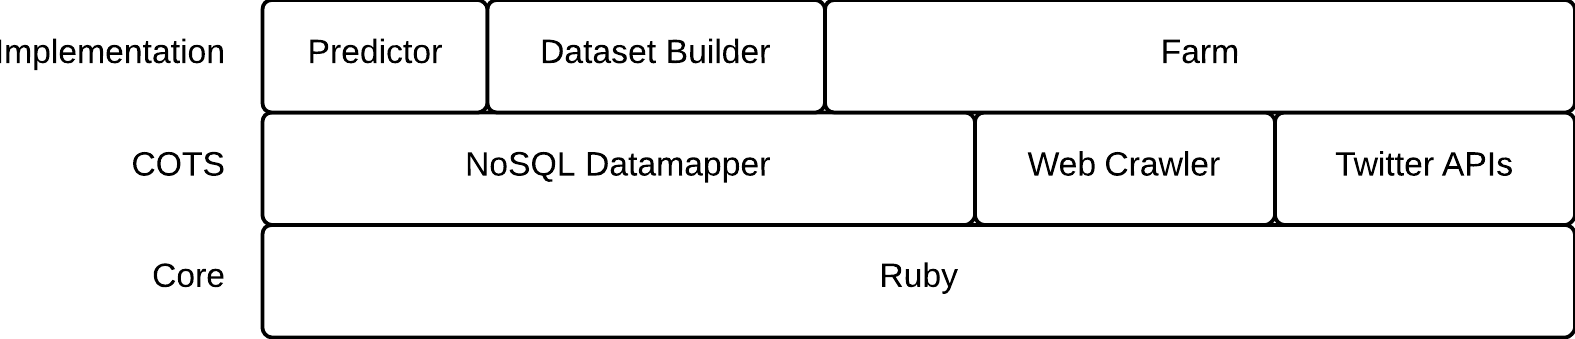
\includegraphics[width=4.5in]{image/architecture-development-view.png}}
\caption{Development view showing the technology stack. Each technology block is dependent on the technology block(s) below it.}
\label{figure:development-view}
\end{figure}

\subsection{Physical View}
The physical view describes the mapping(s) of the software onto hardware, as seen in figure~\ref{figure:development-view}. The NoSQL database communicate with the Twilm implementation. These are both stored on a single computer. This computer has internet access. The Twilm implementation uses the internet access to reach Twitter.

\begin{figure}[H]
\centerline{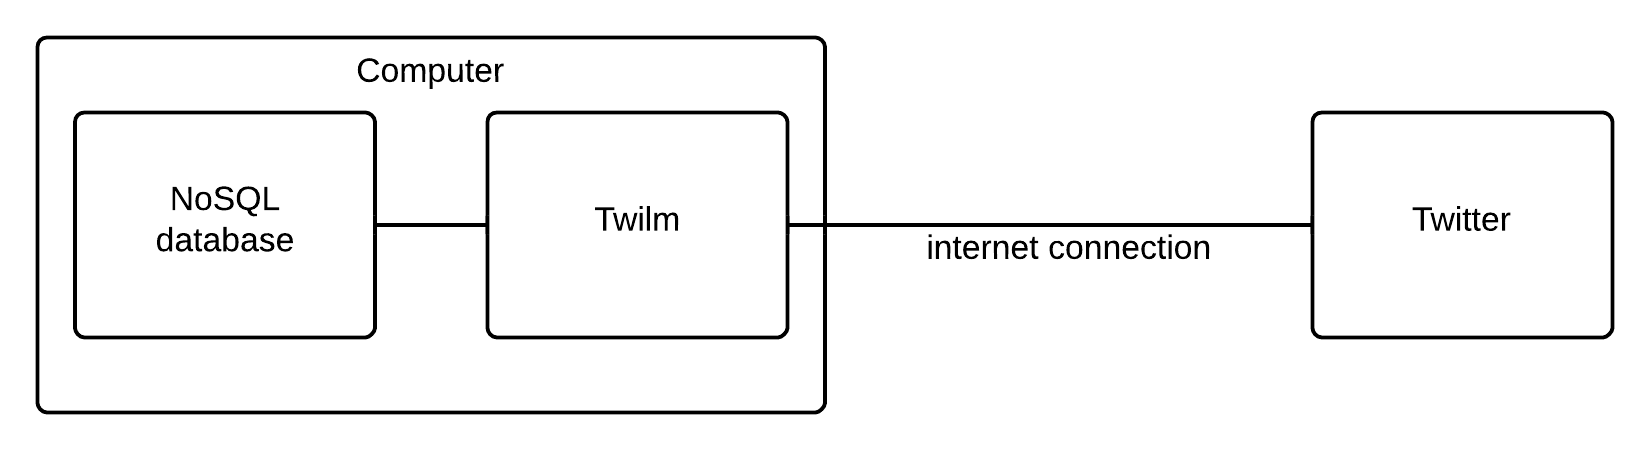
\includegraphics[width=4.5in]{image/architecture-physical-view.png}}
\caption{Physical view showing the components of the system mapped onto hardware. Only a single computer with internet access to Twitter runs the entire system.}
\label{figure:development-view}
\end{figure}

\subsection{Scenarios}

\section{Component Design}


